\begin{figure}[t]
\centering
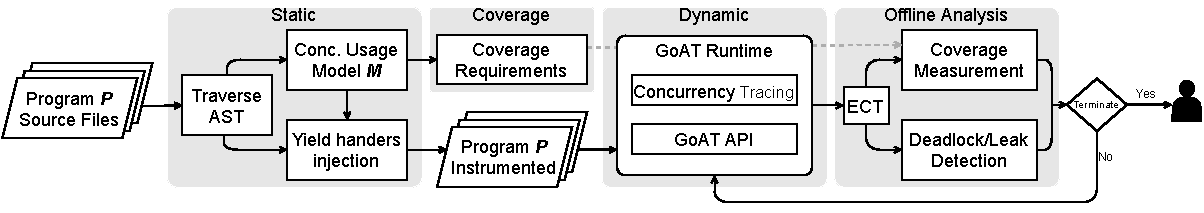
\includegraphics[width=0.99\linewidth]{goat/figs/GOAT_overview.pdf}
%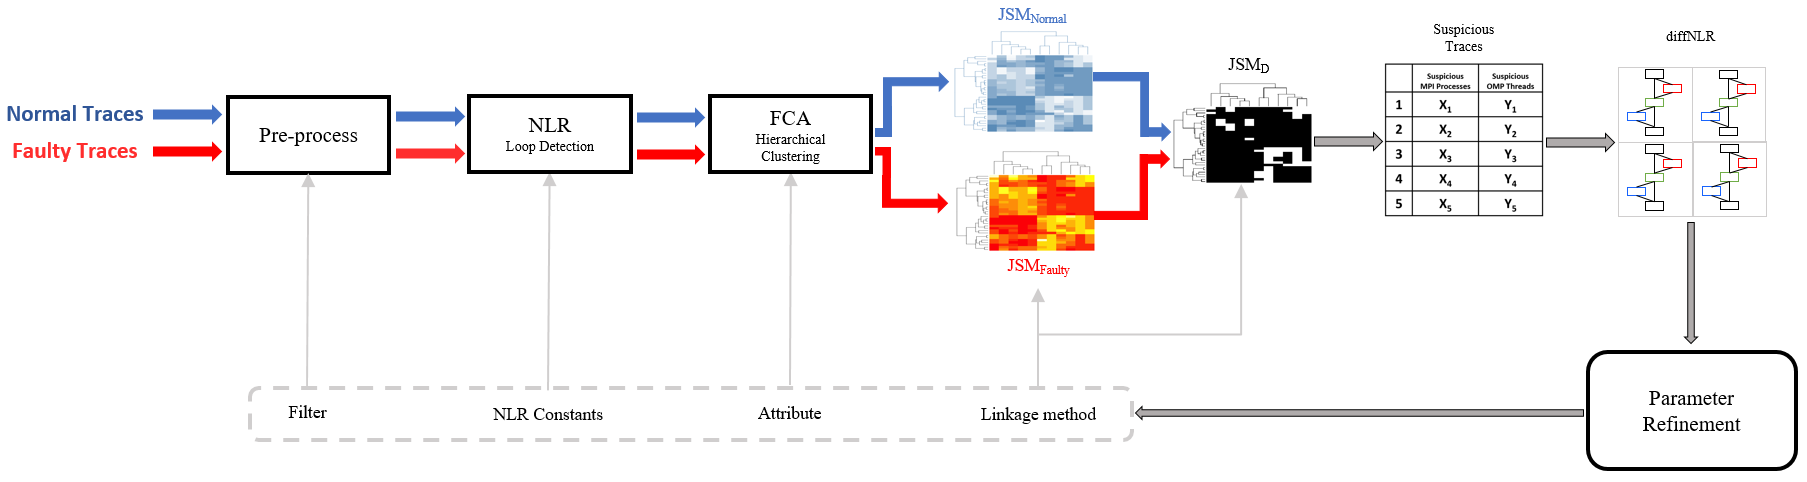
\includegraphics[]{figs/overview.png}
%\includegraphics[]{figs/overv}
\caption{\goat overview}
\label{fig:goat_workflow}
\end{figure}

\begin{listing}[]
\begin{minipage}{.35\textwidth}
\begin{minted}
[
fontsize=\footnotesize,
linenos=true,
escapeinside=||,
breaklines
]
{go}
package main
import "sync"

type Container struct{ |\label{bugListing:containerType_start}|
  sync.Mutex
  stop  chan struct{}
} |\label{bugListing:containerType_end}|

func main() {
  container := &Container{ |\label{bugListing:container_create_start}|
       stop:make(chan struct{})} |\label{bugListing:container_create_end}|
  go Monitor(container) |\label{bugListing:main_go_monitor}|
  go StatusChange(container) |\label{bugListing:main_go_statChange}|
}
\end{minted}
\end{minipage}
\begin{minipage}{.35\textwidth}
\begin{minted}
[
fontsize=\scriptsize,
linenos=true,
escapeinside=||,
breaklines
]
{go}
|\setcounter{FancyVerbLine}{15}|func Monitor(cnt *Container){
  for{
    select{|\label{bugListing:Monitor_select}|
    case <- cnt.stop:  |\label{bugListing:Monitor_case_recv}|
      return |\label{bugListing:Monitor_case_recv_ret}|
    default: |\label{bugListing:Monitor_case_def}|
      cnt.Lock()  |\label{bugListing:Monitor_case_def_lock}|
      cnt.Unlock() |\label{bugListing:Monitor_case_def_unlock}|
}}}
func StatusChange(cnt *Container){
  cnt.Lock() |\label{bugListing:statChange_lock}|
  defer cnt.Unlock() |\label{bugListing:statChange_defer_unlock}|
  cnt.stop <- struct{}{} |\label{bugListing:statChange_send}|
}
\end{minted}
\end{minipage}
\begin{minipage}{.25\textwidth}
  \centering
  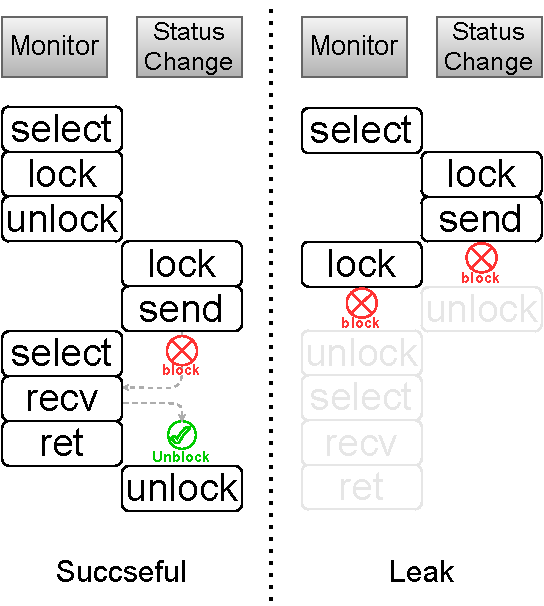
\includegraphics[width=.99\linewidth]{goat/figs/execViz_moby.pdf}
\end{minipage}
\caption{Simplified version of bug \texttt{moby28462}}
\label{listing:moby28462.minipage}
\end{listing}



\begin{table}[]
\centering
\caption{Concurrency usages and coverage requirements of program in listing\ref{listing:moby28462.minipage}}
\scalebox{0.82}{

\begin{tabular}{
>{\columncolor[HTML]{FFFFFF}}c
>{\columncolor[HTML]{FFFFFF}}l |
>{\columncolor[HTML]{FFFFFF}}l |
>{\columncolor[HTML]{FFFFFF}}c |
>{\columncolor[HTML]{FFFFFF}}c |
>{\columncolor[HTML]{FFFFFF}}c |}
\hline
\multicolumn{2}{|c|}{\cellcolor[HTML]{FFFFFF}CU of list. \ref{listing:moby28462.minipage}} & \multicolumn{1}{c|}{\cellcolor[HTML]{FFFFFF}} & \multicolumn{2}{c|}{\cellcolor[HTML]{FFFFFF}Covered by} & \cellcolor[HTML]{FFFFFF} \\ \cline{1-2} \cline{4-5}
\multicolumn{1}{|c|}{\cellcolor[HTML]{FFFFFF}Line} & \multicolumn{1}{c|}{\cellcolor[HTML]{FFFFFF}Kind} & \multicolumn{1}{c|}{\multirow{-2}{*}{\cellcolor[HTML]{FFFFFF}Coverage Requirements}} & run \#1 & run \#2 & \multirow{-2}{*}{\cellcolor[HTML]{FFFFFF}\begin{tabular}[c]{@{}c@{}}Overall\\      Covered\end{tabular}} \\ \hline
\multicolumn{1}{|c|}{\cellcolor[HTML]{FFFFFF}12} & go & covered & $\checkmark_{G0}$ & $\checkmark_{G0}$ & $\checkmark$ \\ \hline
\multicolumn{1}{|c|}{\cellcolor[HTML]{FFFFFF}13} & go & covered & $\checkmark_{G0}$ & $\checkmark_{G0}$ & $\checkmark$ \\ \hline
\multicolumn{1}{|c|}{\cellcolor[HTML]{FFFFFF}} & \cellcolor[HTML]{FFFFFF} & c-recv-blocked & $\checkmark_{G1}$ &  & $\checkmark$ \\ \cline{3-6}
\multicolumn{1}{|c|}{\multirow{-2}{*}{\cellcolor[HTML]{FFFFFF}17}} & \multirow{-2}{*}{\cellcolor[HTML]{FFFFFF}select} & c-recv-unblocking & $\checkmark_{G1}$ &  & $\checkmark$ \\ \hline
\multicolumn{1}{|c|}{\cellcolor[HTML]{FFFFFF}} & \cellcolor[HTML]{FFFFFF} & blocked &  & \cellcolor[HTML]{C0C0C0}$\checkmark_{G1}$ & $\checkmark$ \\ \cline{3-6}
\multicolumn{1}{|c|}{\multirow{-2}{*}{\cellcolor[HTML]{FFFFFF}21}} & \multirow{-2}{*}{\cellcolor[HTML]{FFFFFF}lock} & blocking & $\checkmark_{G1}$ &  & $\checkmark$ \\ \hline
\multicolumn{1}{|c|}{\cellcolor[HTML]{FFFFFF}} & \cellcolor[HTML]{FFFFFF} & unblocking & $\checkmark_{G1}$ &  & $\checkmark$ \\ \cline{3-6}
\multicolumn{1}{|c|}{\multirow{-2}{*}{\cellcolor[HTML]{FFFFFF}22}} & \multirow{-2}{*}{\cellcolor[HTML]{FFFFFF}unlock} & no\_op &  &  &  \\ \hline
\multicolumn{1}{|c|}{\cellcolor[HTML]{FFFFFF}} & \cellcolor[HTML]{FFFFFF} & blocked & $\checkmark_{G2}$ &  & $\checkmark$ \\ \cline{3-6}
\multicolumn{1}{|c|}{\multirow{-2}{*}{\cellcolor[HTML]{FFFFFF}25}} & \multirow{-2}{*}{\cellcolor[HTML]{FFFFFF}lock} & blocking &  & \cellcolor[HTML]{C0C0C0} \textbf{$\checkmark_{G2}$} & $\checkmark$ \\ \hline
\multicolumn{1}{|c|}{\cellcolor[HTML]{FFFFFF}} & \cellcolor[HTML]{FFFFFF} & blocked & $\checkmark_{G2}$ & $\checkmark_{G2}$ & $\checkmark$ \\ \cline{3-6}
\multicolumn{1}{|c|}{\cellcolor[HTML]{FFFFFF}} & \cellcolor[HTML]{FFFFFF} & unblocking &  &  &  \\ \cline{3-6}
\multicolumn{1}{|c|}{\multirow{-3}{*}{\cellcolor[HTML]{FFFFFF}26}} & \multirow{-3}{*}{\cellcolor[HTML]{FFFFFF}send} & no\_op &  &  &  \\ \hline
\multicolumn{1}{|c|}{\cellcolor[HTML]{FFFFFF}} & \cellcolor[HTML]{FFFFFF} & unblocking &  &  &  \\ \cline{3-6}
\multicolumn{1}{|c|}{\multirow{-2}{*}{\cellcolor[HTML]{FFFFFF}27}} & \multirow{-2}{*}{\cellcolor[HTML]{FFFFFF}unlock} & no\_op & $\checkmark_{G2}$ &  & $\checkmark$ \\ \hline
\multicolumn{1}{l}{\cellcolor[HTML]{FFFFFF}} &  & Coverage \% & 60\% & 33\% & 73\% \\ \cline{3-6}
\end{tabular}

}
\label{tab:moby_cov_table}
\end{table}


\begin{figure}[]
\centering
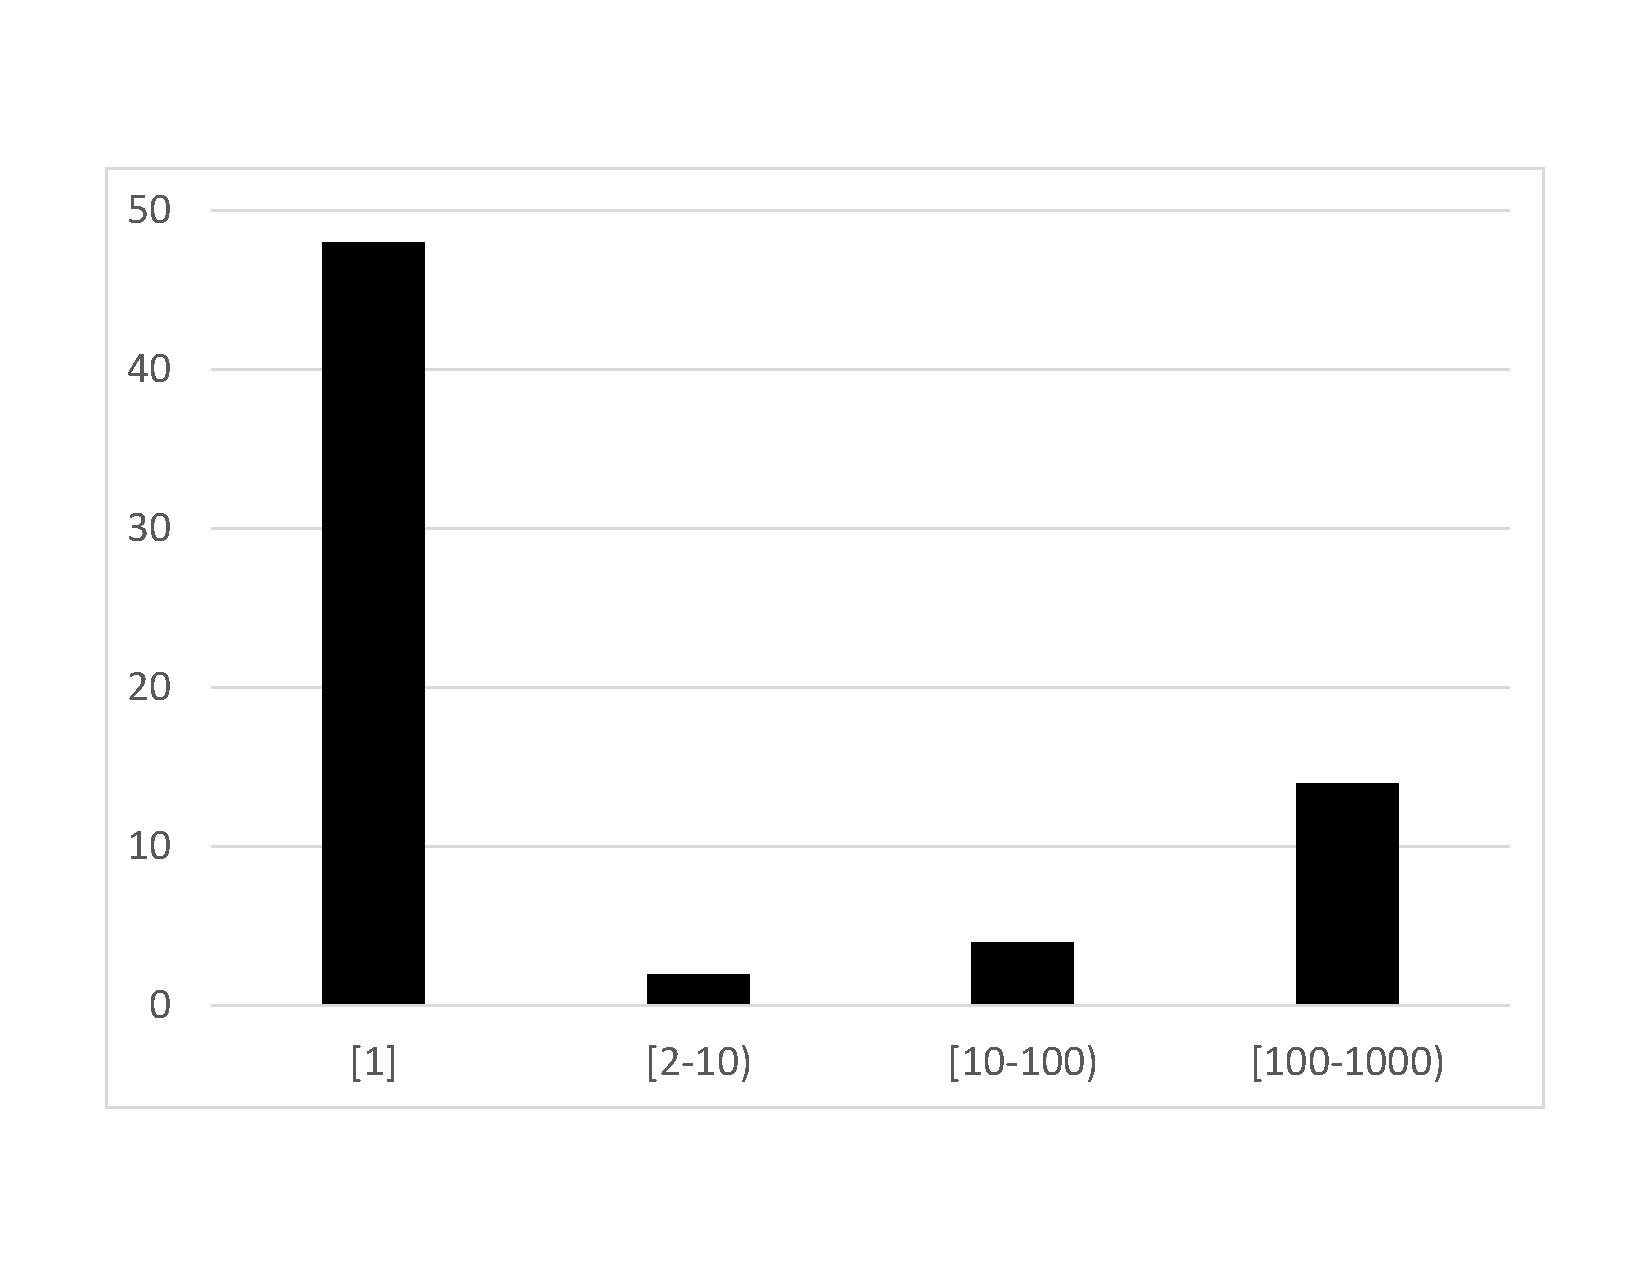
\includegraphics[width=0.6\textwidth]{goat/figs/coverage_motivation.pdf}
%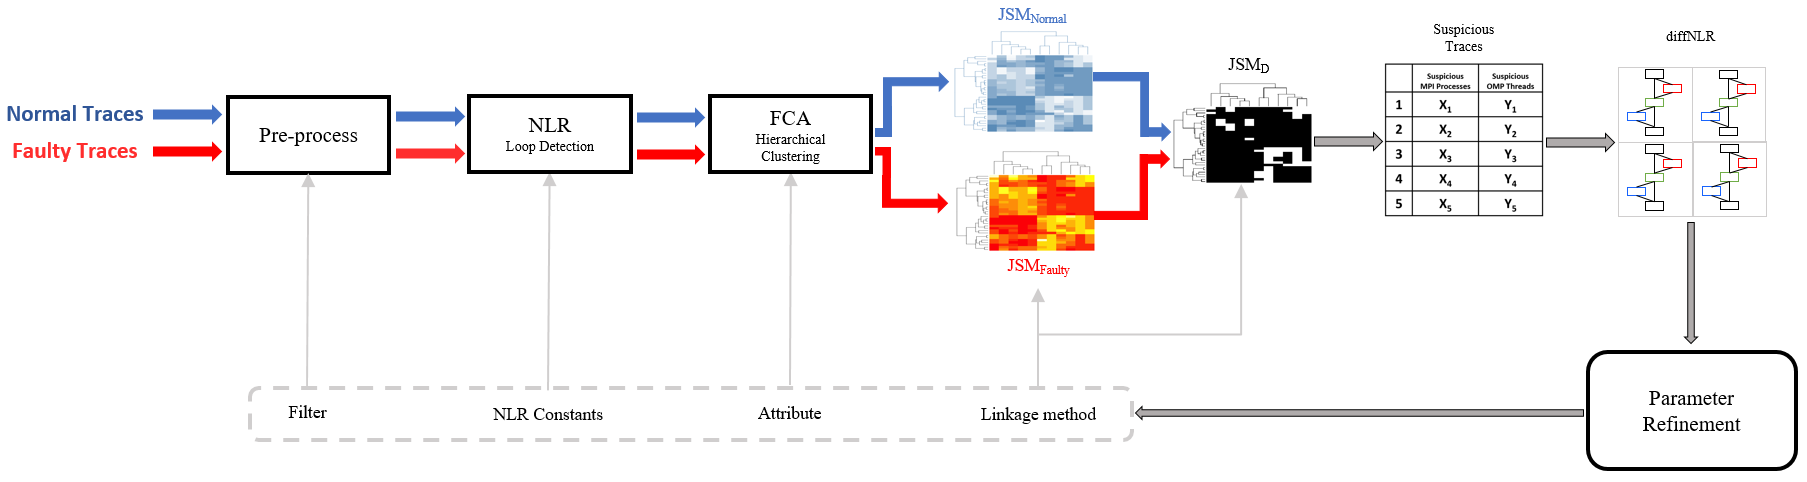
\includegraphics[]{figs/overview.png}
%\includegraphics[]{figs/overv}
\caption{Distribution of number of trials for \goat (D0) to detect 68 blocking bugs in GoKer~\cite{yuan-gobench-cgo21}}
\label{fig:rare_bugs}
\end{figure}






\begin{table}[]
\centering
\caption{Coverge requirements defined for concurrent Go}
\scalebox{0.75}{
\begin{tabular}{|
>{\columncolor[HTML]{FFFFFF}}l |
>{\columncolor[HTML]{FFFFFF}}l |
>{\columncolor[HTML]{FFFFFF}}c |
>{\columncolor[HTML]{FFFFFF}}c |
>{\columncolor[HTML]{FFFFFF}}c |
>{\columncolor[HTML]{FFFFFF}}c |}
\hline
\multicolumn{1}{|c|}{\cellcolor[HTML]{FFFFFF}} & \multicolumn{1}{c|}{\cellcolor[HTML]{FFFFFF}} & \multicolumn{4}{c|}{\cellcolor[HTML]{FFFFFF}Coverage Requirement Types} \\ \cline{3-6}
\multicolumn{1}{|c|}{\multirow{-2}{*}{\cellcolor[HTML]{FFFFFF}\begin{tabular}[c]{@{}c@{}}Coverage\\ Requirements\end{tabular}}} & \multicolumn{1}{c|}{\multirow{-2}{*}{\cellcolor[HTML]{FFFFFF}\begin{tabular}[c]{@{}c@{}}Concurrent\\ Action\end{tabular}}} & Blocked & Unblocking & Blocking & NOP \\ \hline
\cellcolor[HTML]{FFFFFF} & SEND & * & * &  & * \\ \cline{2-6}
\multirow{-2}{*}{\cellcolor[HTML]{FFFFFF}Req. 1: Send/Recv} & RECV & * & * &  & * \\ \hline
\cellcolor[HTML]{FFFFFF} & CASE$_i$ (SEND) & * & * &  & * \\ \cline{2-6}
\multirow{-2}{*}{\cellcolor[HTML]{FFFFFF}Req. 2: Select-Case} & CASE$_i$ (RECV) & * & * &  & * \\ \hline
Req. 3: Lock & LOCK & * &  & * &  \\ \hline
\cellcolor[HTML]{FFFFFF} & CLOSE &  & * &  & * \\ \cline{2-6}
\cellcolor[HTML]{FFFFFF} & UNLOCK &  & * &  & * \\ \cline{2-6}
\cellcolor[HTML]{FFFFFF} & SIGNAL &  & * &  & * \\ \cline{2-6}
\cellcolor[HTML]{FFFFFF} & BRDCST &  & * &  & * \\ \cline{2-6}
\multirow{-5}{*}{\cellcolor[HTML]{FFFFFF}Req. 4: Unblocking} & NB-SELECT &  & * &  & * \\ \hline
Req. 5: Go & Go &  &  &  & * \\ \hline
\end{tabular}

}
\label{tab:cov_req}
\end{table}




\begin{table}[]
    \centering
        \caption{Event categories by the Go execution tracer}
        \begin{tabular}{|l|l|}
        \hline
        \rowcolor[HTML]{C0C0C0}
        \multicolumn{1}{|c|}{\cellcolor[HTML]{C0C0C0}\textbf{Category}} & \multicolumn{1}{c|}{\cellcolor[HTML]{C0C0C0}\textbf{Description}} \\ \hline
        Process & Indication of process/thread start and stop \\ \hline
        GC/Mem & Garbage collection and memory operation events\\ \hline
        Goroutine & Goroutines events: create, block, start, stop, end, etc. \\ \hline
        Syscall & Interactions with system calls \\ \hline
        Users & User annotated regions and tasks (for bounded tracing) \\ \hline
        Misc & System related events like futile wakeup or timers \\ \hline
        \end{tabular}
    \label{tab:events}
\end{table}



\begin{figure}[]
\centering
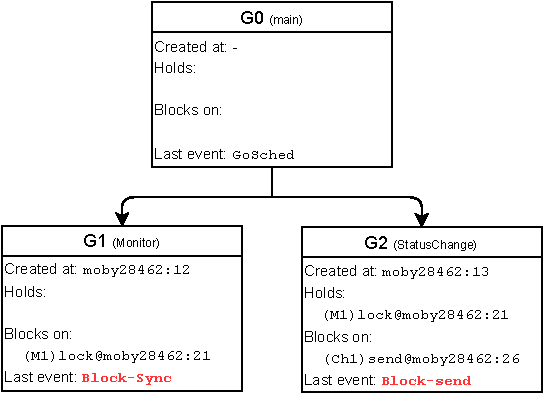
\includegraphics[width=0.75\linewidth]{goat/figs/gtree.pdf}
%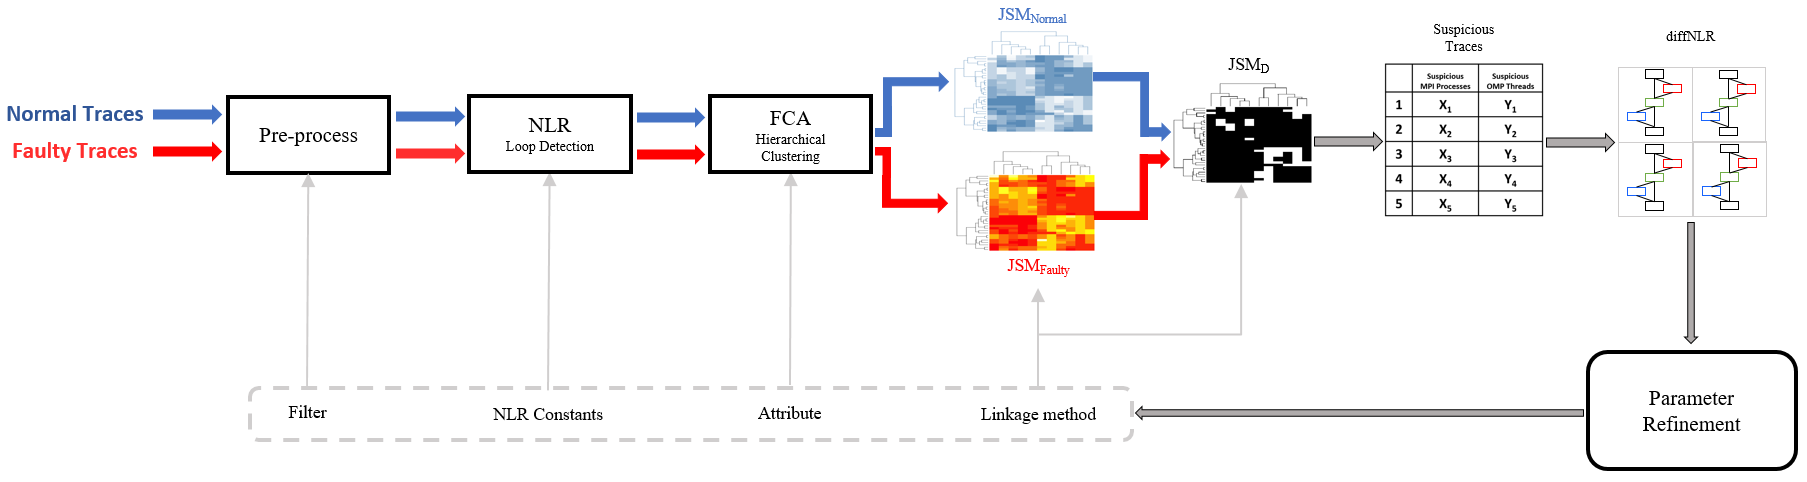
\includegraphics[]{figs/overview.png}
%\includegraphics[]{figs/overv}
\caption{Goroutine tree of the leak situation in listing \ref{listing:moby28462.minipage}}
\label{fig:gtree}
\end{figure}



\begin{small}
\begin{algorithm}[]
 \DontPrintSemicolon
 \SetKwFunction{KwDeadlockCheck}{DeadlockCheck}
% \SetKwInOut{Input}{Input} \SetKwInOut{Output}{Output}\SetKwInOut{Local}{Local}
  %\SetKw{KwEach}{each}
 %\Input{Stack of elements $S$, $S[1]$ is top}
 %\Output{$NLR(T)$}
 \KwDeadlockCheck{$G$}:{\\
 \Indp
    \If{$cur$.lastEvent$ \neq$ \texttt{GoSched}}{
      return \textbf{Global Deadlock}\;
    }
    $toVisit$ = $[G.children]$\;
    \For{ $|toVisit| \neq 0$}{
         $cur$ = $toVisit$[0]\;
         \If{$cur$.lastEvent $\neq$ \texttt{GoEnd}}{
            return \textbf{Partial Deadlock (leak)}\;
          }
         \For {$n$ in $cur.Children$}{
            append $n$ to $toVisit$\;
          }
          $toVisit = toVisit[1:]$\;
      }
      return \textbf{Pass}\;
  }
 \caption{\texttt{DeadlockCheck} procedure with root node of goroutine tree (main goroutine) as input}
 \label{proc:deadlockCheck}
\end{algorithm}
\end{small}


\begin{table}[]
\caption{Output of each tool on GoKer \cite{yuan-gobench-cgo21} blocking bugs. Detected bug (minimum \# of executions required) -- \textbf{X (1000)}: the tool is not able to detect any bug after 1000 executions. \textbf{PDL}: Partial Deadlock, \textbf{GDL}: Global Deadlock, \textbf{PDL-k}: Partial Deadlock with \textit{k} number of goroutines leaked. \textbf{DL}: A warning for potential deadlock is issued. \textbf{TO/GDL}: The global deadlock is detected because none of goroutines made any progress after 30 seconds, \textbf{CRASH}: The execution paniced because of a flaw in the execution (e.g., send on closed channel panic), \textbf{HANG}: The tool halt for more than 10 minutes.}
\centering
\scalebox{0.46}{
    % Please add the following required packages to your document preamble:
% \usepackage{multirow}
% \usepackage[table,xcdraw]{xcolor}
% If you use beamer only pass "xcolor=table" option, i.e. \documentclass[xcolor=table]{beamer}
\begin{tabular}{|c|c|c|ccc|ccccc|}
\hline
\multicolumn{3}{|c|}{Bug Description} & \multicolumn{8}{c|}{Debugging Tools} \\ \hline
 &  &  & \multicolumn{1}{c|}{} & \multicolumn{1}{c|}{} &  & \multicolumn{5}{c|}{GOAT} \\ \cline{7-11}
\multirow{-2}{*}{Cause} & \multirow{-2}{*}{SubCause} & \multirow{-2}{*}{Bug ID} & \multicolumn{1}{c|}{\multirow{-2}{*}{BUILTINDL}} & \multicolumn{1}{c|}{\multirow{-2}{*}{GOLEAK}} & \multirow{-2}{*}{LOCKDL} & \multicolumn{1}{c|}{D0} & \multicolumn{1}{c|}{D1} & \multicolumn{1}{c|}{D2} & \multicolumn{1}{c|}{D3} & D4 \\ \hline
 &  & cockroach\_2448 & X (1000) & X (1000) & X (1000) & CRASH (1) & CRASH (1) & CRASH (1) & CRASH (1) & CRASH (1) \\ \cline{3-3}
 &  & cockroach\_24808 & GDL (1) & GDL (1) & TO/GDL (1) & TO/GDL (1) & TO/GDL (1) & TO/GDL (1) & TO/GDL (1) & TO/GDL (1) \\ \cline{3-3}
 &  & cockroach\_25456 & GDL (1) & GDL(1) & TO/GDL (1) & TO/GDL (1) & TO/GDL (1) & TO/GDL (1) & TO/GDL (1) & TO/GDL (1) \\ \cline{3-3}
 &  & cockroach\_35073 & GDL (1) & GDL (1) & TO/GDL (1) & TO/GDL (1) & TO/GDL (1) & TO/GDL (1) & TO/GDL (1) & TO/GDL (1) \\ \cline{3-3}
 &  & cockroach\_35931 & GDL (1) & GDL (1) & TO/GDL (1) & TO/GDL (1) & TO/GDL (1) & TO/GDL (1) & TO/GDL (1) & TO/GDL (1) \\ \cline{3-3}
 &  & etcd\_6857 & X (1000) & PDL (325) & X (1000) & \cellcolor[HTML]{EFEFEF}PDL-1 (1) & \cellcolor[HTML]{EFEFEF}PDL-1 (1) & \cellcolor[HTML]{EFEFEF}PDL-1 (11) & \cellcolor[HTML]{EFEFEF}PDL-1 (3) & \cellcolor[HTML]{EFEFEF}PDL-1 (3) \\ \cline{3-3}
 &  & grpc\_1275 & X (1000) & PDL (1) & X (1000) & PDL-1 (1) & PDL-1 (1) & PDL-1 (1) & PDL-1 (1) & PDL-1 (1) \\ \cline{3-3}
 &  & grpc\_1424 & X (1000) & PDL (1) & X (1000) & PDL-1 (1) & PDL-1 (1) & PDL-1 (1) & PDL-1 (1) & PDL-1 (1) \\ \cline{3-3}
 &  & grpc\_660 & X (1000) & PDL (1) & X (1000) & PDL-1 (1) & PDL-1 (1) & PDL-1 (1) & PDL-1 (1) & PDL-1 (1) \\ \cline{3-3}
 &  & istio\_17860 & X (1000) & PDL (1) & X (1000) & PDL-1 (2) & PDL-1 (1) & PDL-1 (1) & PDL-1 (1) & PDL-1 (1) \\ \cline{3-3}
 &  & kubernetes\_38669 & X (1000) & PDL (1) & X (1000) & PDL-1 (1) & PDL-1 (1) & PDL-1 (1) & PDL-1 (1) & PDL-1 (1) \\ \cline{3-3}
 &  & kubernetes\_5316 & X (1000) & PDL (1) & X (1000) & PDL-1 (1) & PDL-2 (1) & PDL-1 (1) & PDL-2 (1) & PDL-2 (1) \\ \cline{3-3}
 &  & kubernetes\_70277 & GDL (1) & GDL (1) & TO/GDL (1) & TO/GDL (1) & TO/GDL (1) & TO/GDL (1) & TO/GDL (1) & TO/GDL (1) \\ \cline{3-3}
 &  & moby\_21233 & X (1000) & PDL (1) & X (1000) & PDL-2 (1) & PDL-2 (1) & PDL-2 (1) & PDL-2 (1) & PDL-2 (1) \\ \cline{3-3}
 &  & moby\_33293 & X (1000) & PDL (1) & X (1000) & PDL-1 (1) & PDL-1 (3) & PDL-1 (1) & PDL-1 (1) & PDL-1 (1) \\ \cline{3-3}
 &  & moby\_4395 & X (1000) & PDL (1) & X (1000) & PDL-1 (1) & PDL-1 (1) & PDL-1 (1) & PDL-1 (1) & PDL-1 (1) \\ \cline{3-3}
 & \multirow{-17}{*}{Channel} & syncthing\_5795 & GDL (1) & GDL (1) & TO/GDL (1) & TO/GDL (1) & TO/GDL (1) & TO/GDL (1) & TO/GDL (1) & TO/GDL (1) \\ \cline{2-11}
 &  & kubernetes\_11298 & X (1000) & X (1000) & TO/GDL (179) & X (1000) & TO/GDL (352) & TO/GDL (158) & TO/GDL (179) & TO/GDL (179) \\ \cline{3-3}
 & \multirow{-2}{*}{\begin{tabular}[c]{@{}c@{}}Channel   \&\\      Conditional Variable\end{tabular}} & moby\_27782 & X (1000) & PDL (741) & X (1000) & X (1000) & \cellcolor[HTML]{EFEFEF}PDL-2 (1) & \cellcolor[HTML]{EFEFEF}PDL-2 (1) & \cellcolor[HTML]{EFEFEF}PDL-2 (4) & \cellcolor[HTML]{EFEFEF}PDL-2 (4) \\ \cline{2-11}
 &  & cockroach\_10790 & X (1000) & PDL (3) & X (1000) & PDL-2 (1) & PDL-2 (1) & PDL-2 (1) & PDL-2 (1) & PDL-2 (1) \\ \cline{3-3}
 &  & cockroach\_13197 & X (1000) & PDL (1) & X (1000) & PDL-1 (1) & PDL-1 (1) & PDL-1 (1) & PDL-1 (1) & PDL-1 (1) \\ \cline{3-3}
 &  & cockroach\_13755 & X (1000) & PDL (1) & X (1000) & PDL-1 (1) & PDL-1 (1) & PDL-1 (1) & PDL-1 (1) & PDL-1 (1) \\ \cline{3-3}
 &  & cockroach\_18101 & X (1000) & PDL (1) & X (1000) & PDL-1 (1) & PDL-1 (1) & PDL-1 (1) & PDL-1 (1) & PDL-1 (1) \\ \cline{3-3}
 &  & grpc\_862 & X (1000) & PDL (1) & X (1000) & PDL-1 (1) & PDL-1 (1) & PDL-1 (1) & PDL-1 (1) & PDL-1 (1) \\ \cline{3-3}
 &  & istio\_18454 & X (1000) & PDL (13) & X (1000) & PDL-2 (5) & PDL-1 (14) & PDL-1 (4) & PDL-1 (6) & PDL-1 (6) \\ \cline{3-3}
 &  & kubernetes\_25331 & X (1000) & PDL (1) & X (1000) & PDL-1 (1) & PDL-1 (1) & PDL-1 (1) & PDL-1 (1) & PDL-1 (1) \\ \cline{3-3}
 & \multirow{-8}{*}{\begin{tabular}[c]{@{}c@{}}Channel \& \\      Context\end{tabular}} & moby\_33781 & X (1000) & PDL (1) & X (1000) & PDL-1 (221) & PDL-1 (10) & PDL-1 (8) & PDL-1 (10) & PDL-1 (10) \\ \cline{2-11}
 &  & moby\_29733 & GDL (1) & GDL (1) & TO/GDL (1) & TO/GDL (1) & TO/GDL (1) & TO/GDL (1) & TO/GDL (1) & TO/GDL (1) \\ \cline{3-3}
\multirow{-29}{*}{\begin{tabular}[c]{@{}c@{}}Communication\\       Deadlock\end{tabular}} & \multirow{-2}{*}{Condition Variable} & moby\_30408 & GDL (1) & GDL (1) & TO/GDL (1) & TO/GDL (1) & TO/GDL (1) & TO/GDL (1) & TO/GDL (1) & TO/GDL (1) \\ \hline
 &  & etcd\_6873 & X (1000) & PDL (371) & X (1000) & PDL-2 (1) & PDL-2 (2) & PDL-2 (7) & PDL-2 (6) & PDL-2 (6) \\ \cline{3-3}
 &  & etcd\_7443 & X (1000) & X (1000) & X (1000) & X (1000) & \cellcolor[HTML]{EFEFEF}PDL-1 (9) & \cellcolor[HTML]{EFEFEF}PDL-1 (15) & \cellcolor[HTML]{EFEFEF}PDL-1 (14) & \cellcolor[HTML]{EFEFEF}PDL-1 (14) \\ \cline{3-3}
 &  & etcd\_7492 & HANG (1) & HANG (1) & TO/GDL (4) & TO/GDL (1) & TO/GDL (1) & TO/GDL (1) & TO/GDL (1) & TO/GDL (1) \\ \cline{3-3}
 &  & etcd\_7902 & X (1000) & PDL (1) & X (1000) & PDL-4 (1) & PDL-4 (1) & PDL-4 (1) & PDL-4 (1) & PDL-4 (1) \\ \cline{3-3}
 &  & grpc\_1353 & X (1000) & PDL (1) & X (1000) & CRASH (1) & CRASH (1) & PDL-3 (1) & PDL-3 (1) & PDL-3 (1) \\ \cline{3-3}
 &  & grpc\_1460 & X (1000) & PDL (1) & X (1000) & PDL-2 (135) & PDL-2 (1) & PDL-2 (2) & PDL-2 (1) & PDL-2 (1) \\ \cline{3-3}
 &  & istio\_16224 & GDL (1) & GDL (1) & TO/GDL (1) & TO/GDL (1) & TO/GDL (1) & TO/GDL (1) & TO/GDL (1) & TO/GDL (1) \\ \cline{3-3}
 &  & kubernetes\_10182 & X (1000) & PDL (44) & X (1000) & \cellcolor[HTML]{EFEFEF}PDL-2 (1) & \cellcolor[HTML]{EFEFEF}PDL-2 (1) & \cellcolor[HTML]{EFEFEF}PDL-2 (1) & \cellcolor[HTML]{EFEFEF}PDL-2 (1) & \cellcolor[HTML]{EFEFEF}PDL-2 (1) \\ \cline{3-3}
 &  & kubernetes\_1321 & X (1000) & PDL (307) & X (1000) & X (1000) & \cellcolor[HTML]{EFEFEF}PDL-1 (1) & \cellcolor[HTML]{EFEFEF}PDL-1 (1) & \cellcolor[HTML]{EFEFEF}PDL-1 (1) & \cellcolor[HTML]{EFEFEF}PDL-1 (1) \\ \cline{3-3}
 &  & kubernetes\_26980 & GDL (375) & GDL (131) & X (1000) & TO/GDL (191) & TO/GDL (1) & TO/GDL (1) & TO/GDL (1) & TO/GDL (1) \\ \cline{3-3}
 &  & kubernetes\_6632 & X (1000) & X (1000) & X (1000) & \cellcolor[HTML]{EFEFEF}PDL-2 (1) & \cellcolor[HTML]{EFEFEF}PDL-2 (1) & \cellcolor[HTML]{EFEFEF}PDL-2 (2) & \cellcolor[HTML]{EFEFEF}PDL-2 (1) & \cellcolor[HTML]{EFEFEF}PDL-2 (1) \\ \cline{3-3}
 &  & moby\_28462 & X (1000) & PDL (5) & X (1000) & PDL-2 (39) & PDL-2 (1) & PDL-2 (1) & PDL-2 (1) & PDL-2 (1) \\ \cline{3-3}
 & \multirow{-13}{*}{Channel \& Lock} & serving\_2137 & X (1000) & X (1000) & X (1000) & X (1000) & X (1000) & TO/GDL (88) & X (1000) & X (1000) \\ \cline{2-11}
 &  & cockroach\_1055 & GDL (1) & GDL (1) & TO/GDL (1) & TO/GDL (1) & TO/GDL (1) & TO/GDL (1) & TO/GDL (1) & TO/GDL (1) \\ \cline{3-3}
 & \multirow{-2}{*}{\begin{tabular}[c]{@{}c@{}}Channel   \& \\      WaitGroup\end{tabular}} & cockroach\_1462 & X (1000) & X (1000) & TO/GDL (1) & X (1000) & TO/GDL (1) & TO/GDL (1) & TO/GDL (1) & TO/GDL (1) \\ \cline{2-11}
\multirow{-16}{*}{\begin{tabular}[c]{@{}c@{}}Mixed \\      Deadlock\end{tabular}} & Misuse WaitGroup & moby\_25384 & X (1000) & PDL (1) & X (1000) & PDL-1 (1) & PDL-1 (1) & PDL-1 (1) & PDL-1 (1) & PDL-1 (1) \\ \hline
 &  & cockroach\_584 & X (1000) & PDL (1) & X (1000) & PDL-1 (1) & PDL-1 (1) & PDL-1 (1) & PDL-1 (1) & PDL-1 (1) \\ \cline{3-3}
 &  & cockroach\_9935 & X (1000) & PDL (1) & DL (721) & PDL-1 (1) & PDL-1 (2) & PDL-1 (1) & PDL-1 (1) & PDL-1 (1) \\ \cline{3-3}
 &  & etcd\_10492 & GDL (1) & GDL (1) & DL (1) & TO/GDL (1) & TO/GDL (1) & TO/GDL (1) & TO/GDL (1) & TO/GDL (1) \\ \cline{3-3}
 &  & etcd\_5509 & X (1000) & GDL (766) & TO/GDL (426) & X (1000) & TO/GDL (1) & TO/GDL (1) & TO/GDL (1) & TO/GDL (1) \\ \cline{3-3}
 &  & etcd\_6708 & GDL (1) & GDL (1) & DL (1) & TO/GDL (1) & TO/GDL (1) & TO/GDL (1) & TO/GDL (1) & TO/GDL (1) \\ \cline{3-3}
 &  & grpc\_3017 & GDL (4) & GDL (4) & TO/GDL (3) & TO/GDL (1) & TO/GDL (1) & TO/GDL (1) & TO/GDL (1) & TO/GDL (1) \\ \cline{3-3}
 &  & grpc\_795 & GDL (1) & GDL (1) & DL (1) & TO/GDL (1) & TO/GDL (1) & TO/GDL (1) & TO/GDL (1) & TO/GDL (1) \\ \cline{3-3}
 &  & hugo\_5379 & GDL (1) & GDL (1) & TO/GDL (1) & TO/GDL (1) & TO/GDL (1) & TO/GDL (1) & TO/GDL (1) & TO/GDL (1) \\ \cline{3-3}
 &  & moby\_17176 & X (1000) & PDL (1) & X (1000) & PDL-1 (1) & PDL-1 (1) & PDL-1 (1) & PDL-1 (1) & PDL-1 (1) \\ \cline{3-3}
 &  & moby\_36114 & X (1000) & PDL (1) & X (1000) & PDL-1 (1) & PDL-1 (1) & PDL-1 (1) & PDL-1 (1) & PDL-1 (1) \\ \cline{3-3}
 &  & moby\_7559 & X (1000) & PDL (1) & X (1000) & PDL-1 (1) & PDL-1 (1) & PDL-1 (1) & PDL-1 (1) & PDL-1 (1) \\ \cline{3-3}
 & \multirow{-12}{*}{Double locking} & syncthing\_4829 & GDL (1) & GDL (1) & DL (1) & TO/GDL (1) & TO/GDL (1) & TO/GDL (1) & TO/GDL (1) & TO/GDL (1) \\ \cline{2-11}
 &  & cockroach\_16167 & X (1000) & X (1000) & DL (1) & X (1000) & TO/GDL (1) & TO/GDL (1) & TO/GDL (1) & TO/GDL (1) \\ \cline{3-3}
 &  & cockroach\_3710 & X (1000) & X (1000) & DL (123) & \cellcolor[HTML]{EFEFEF}PDL-2 (28) & \cellcolor[HTML]{EFEFEF}PDL-2 (1) & \cellcolor[HTML]{EFEFEF}PDL-2 (1) & \cellcolor[HTML]{EFEFEF}PDL-2 (1) & \cellcolor[HTML]{EFEFEF}PDL-2 (1) \\ \cline{3-3}
 &  & cockroach\_6181 & X (1000) & PDL (1) & X (1000) & PDL-4 (1) & PDL-4 (1) & PDL-3 (1) & PDL-1 (1) & PDL-1 (1) \\ \cline{3-3}
 &  & hugo\_3251 & GDL (1) & GDL (1) & DL (1) & TO/GDL (1) & TO/GDL (1) & TO/GDL (1) & TO/GDL (1) & TO/GDL (1) \\ \cline{3-3}
 &  & kubernetes\_58107 & X (1000) & X (1000) & X (1000) & \cellcolor[HTML]{EFEFEF}PDL-1 (1) & \cellcolor[HTML]{EFEFEF}PDL-1 (1) & \cellcolor[HTML]{EFEFEF}PDL-1 (1) & \cellcolor[HTML]{EFEFEF}PDL-1 (1) & \cellcolor[HTML]{EFEFEF}PDL-1 (1) \\ \cline{3-3}
 & \multirow{-6}{*}{RWR deadlock} & kubernetes\_62464 & X (1000) & X (1000) & DL (6) & PDL-2 (161) & PDL-2 (7) & PDL-2 (2) & PDL-2 (3) & PDL-2 (3) \\ \cline{2-11}
 &  & cockroach\_10214 & X (1000) & X (1000) & X (1000) & \cellcolor[HTML]{EFEFEF}PDL-2 (368) & \cellcolor[HTML]{EFEFEF}PDL-2 (1) & \cellcolor[HTML]{EFEFEF}PDL-2 (1) & \cellcolor[HTML]{EFEFEF}PDL-2 (1) & \cellcolor[HTML]{EFEFEF}PDL-2 (1) \\ \cline{3-3}
 &  & cockroach\_7504 & X (1000) & X (1000) & X (1000) & \cellcolor[HTML]{EFEFEF}PDL-2 (199) & \cellcolor[HTML]{EFEFEF}PDL-2 (1) & \cellcolor[HTML]{EFEFEF}PDL-2 (7) & \cellcolor[HTML]{EFEFEF}PDL-2 (1) & \cellcolor[HTML]{EFEFEF}PDL-2 (1) \\ \cline{3-3}
 &  & kubernetes\_13135 & X (1000) & PDL (1) & DL (4) & PDL-2 (1) & PDL-2 (5) & PDL-2 (1) & PDL-2 (22) & PDL-2 (22) \\ \cline{3-3}
 &  & kubernetes\_30872 & X (1000) & PDL (338) & X (1000) & \cellcolor[HTML]{EFEFEF}PDL-3 (50) & \cellcolor[HTML]{EFEFEF}PDL-3 (2) & \cellcolor[HTML]{EFEFEF}PDL-3 (1) & \cellcolor[HTML]{EFEFEF}PDL-3 (6) & \cellcolor[HTML]{EFEFEF}PDL-3 (6) \\ \cline{3-3}
\multirow{-23}{*}{\begin{tabular}[c]{@{}c@{}}Resource \\      Deadlock\end{tabular}} & \multirow{-5}{*}{AB-BA deadlock} & moby\_4951 & X (1000) & PDL (120) & X (1000) & \cellcolor[HTML]{EFEFEF}PDL-2 (15) & \cellcolor[HTML]{EFEFEF}PDL-2 (2) & \cellcolor[HTML]{EFEFEF}PDL-2 (2) & \cellcolor[HTML]{EFEFEF}PDL-2 (1) & \cellcolor[HTML]{EFEFEF}PDL-2 (1) \\ \hline
\multicolumn{1}{|l|}{Total Bugs:} & \multicolumn{1}{l|}{68} & \multicolumn{1}{l|}{Total Detected:} & 19 & 56 & 26 & 60 & 67 & 68 & 67 & 67 \\ \hline
\end{tabular}

  }
\label{tab:comparison}
\end{table}

\begin{figure}
\centering
  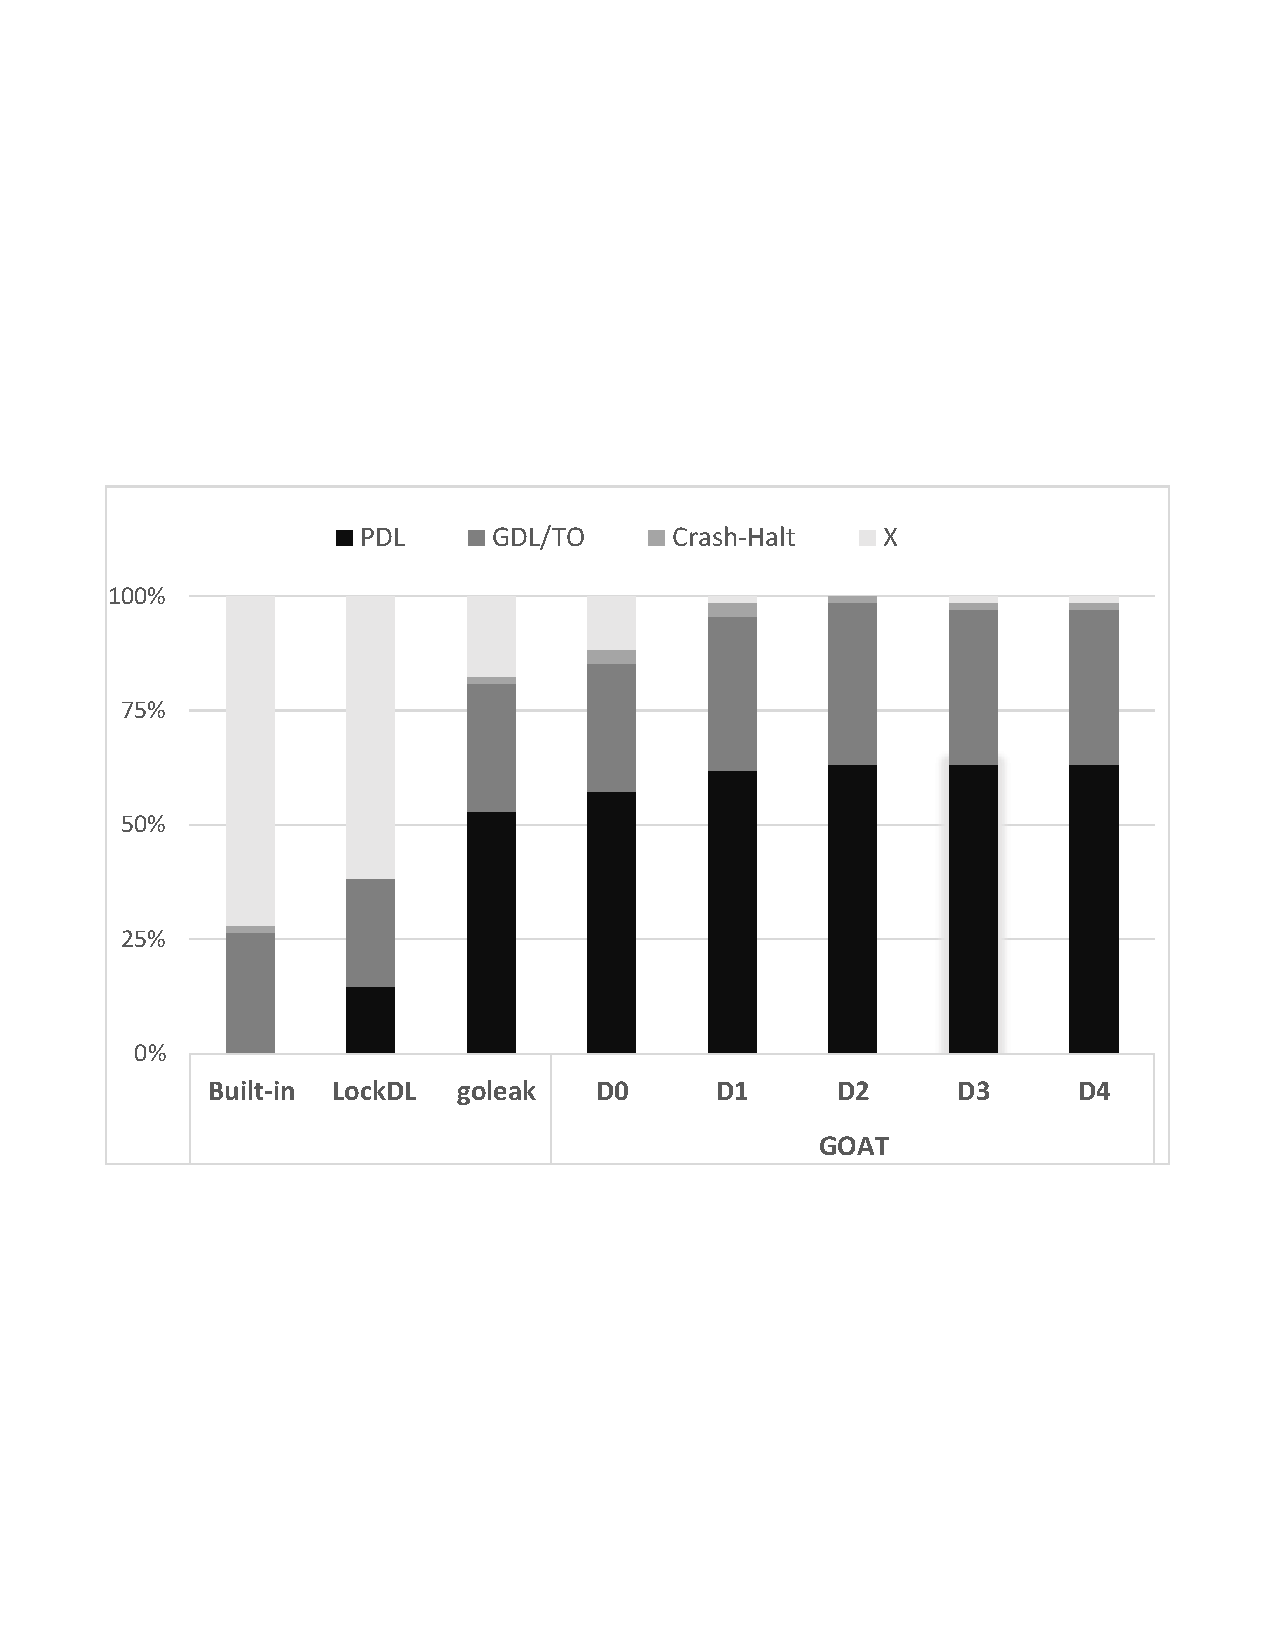
\includegraphics[width=.85\linewidth]{goat/figs/P4_detections.pdf}
  \caption{Histogram of detected bugs by each tool performed on 68 GoKer blocking bugs. PDL: partial deadlock, GDL/TO: global deadlock, Crash/Halt: causes the program to crash or halt during detection.}
  \label{fig:detection}
\end{figure}


\begin{figure}
\centering
  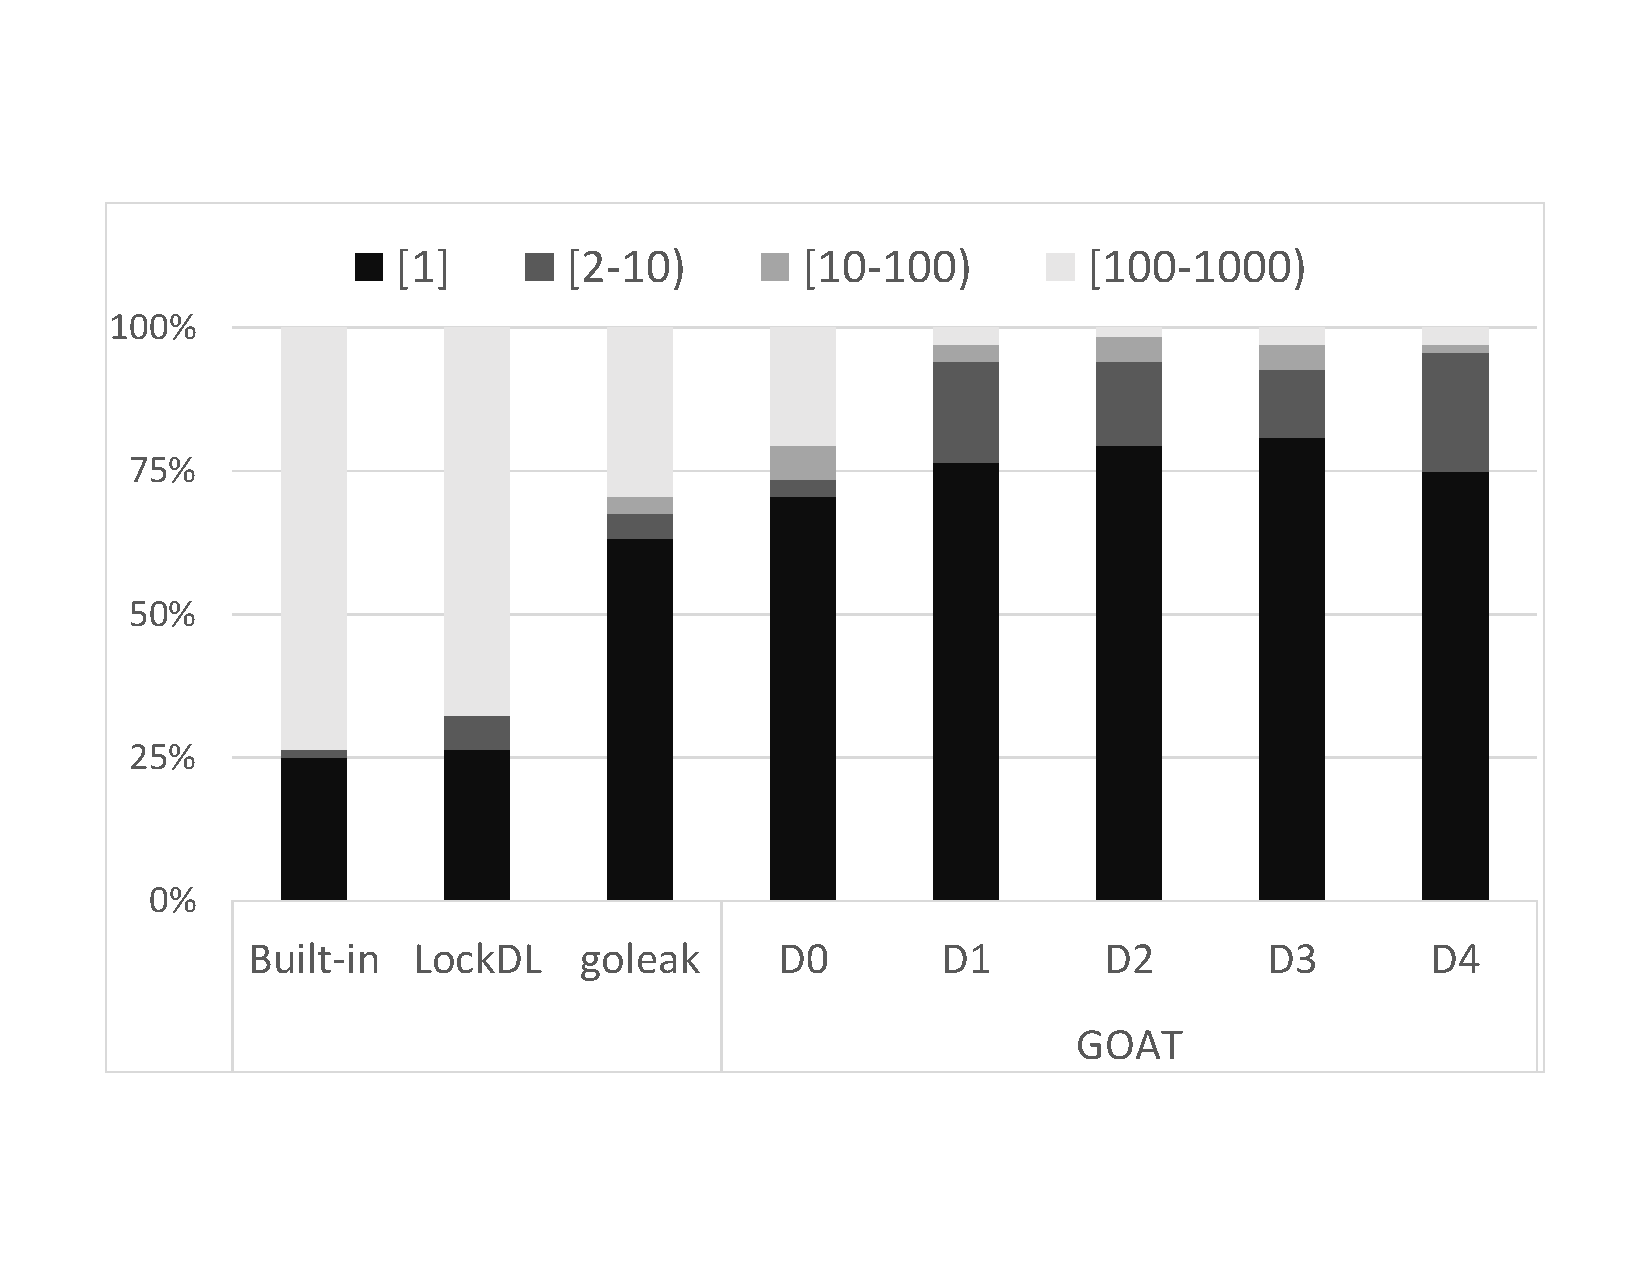
\includegraphics[width=.85\linewidth]{goat/figs/P4_runs2.pdf}
  \caption{Percentage distribution for the average required number of iterations (falling into each of the four given intervals) by each tool to detect 68 GoKer blocking bugs.}
  \label{fig:runs}
\end{figure}





\begin{figure}[]
   \centering
   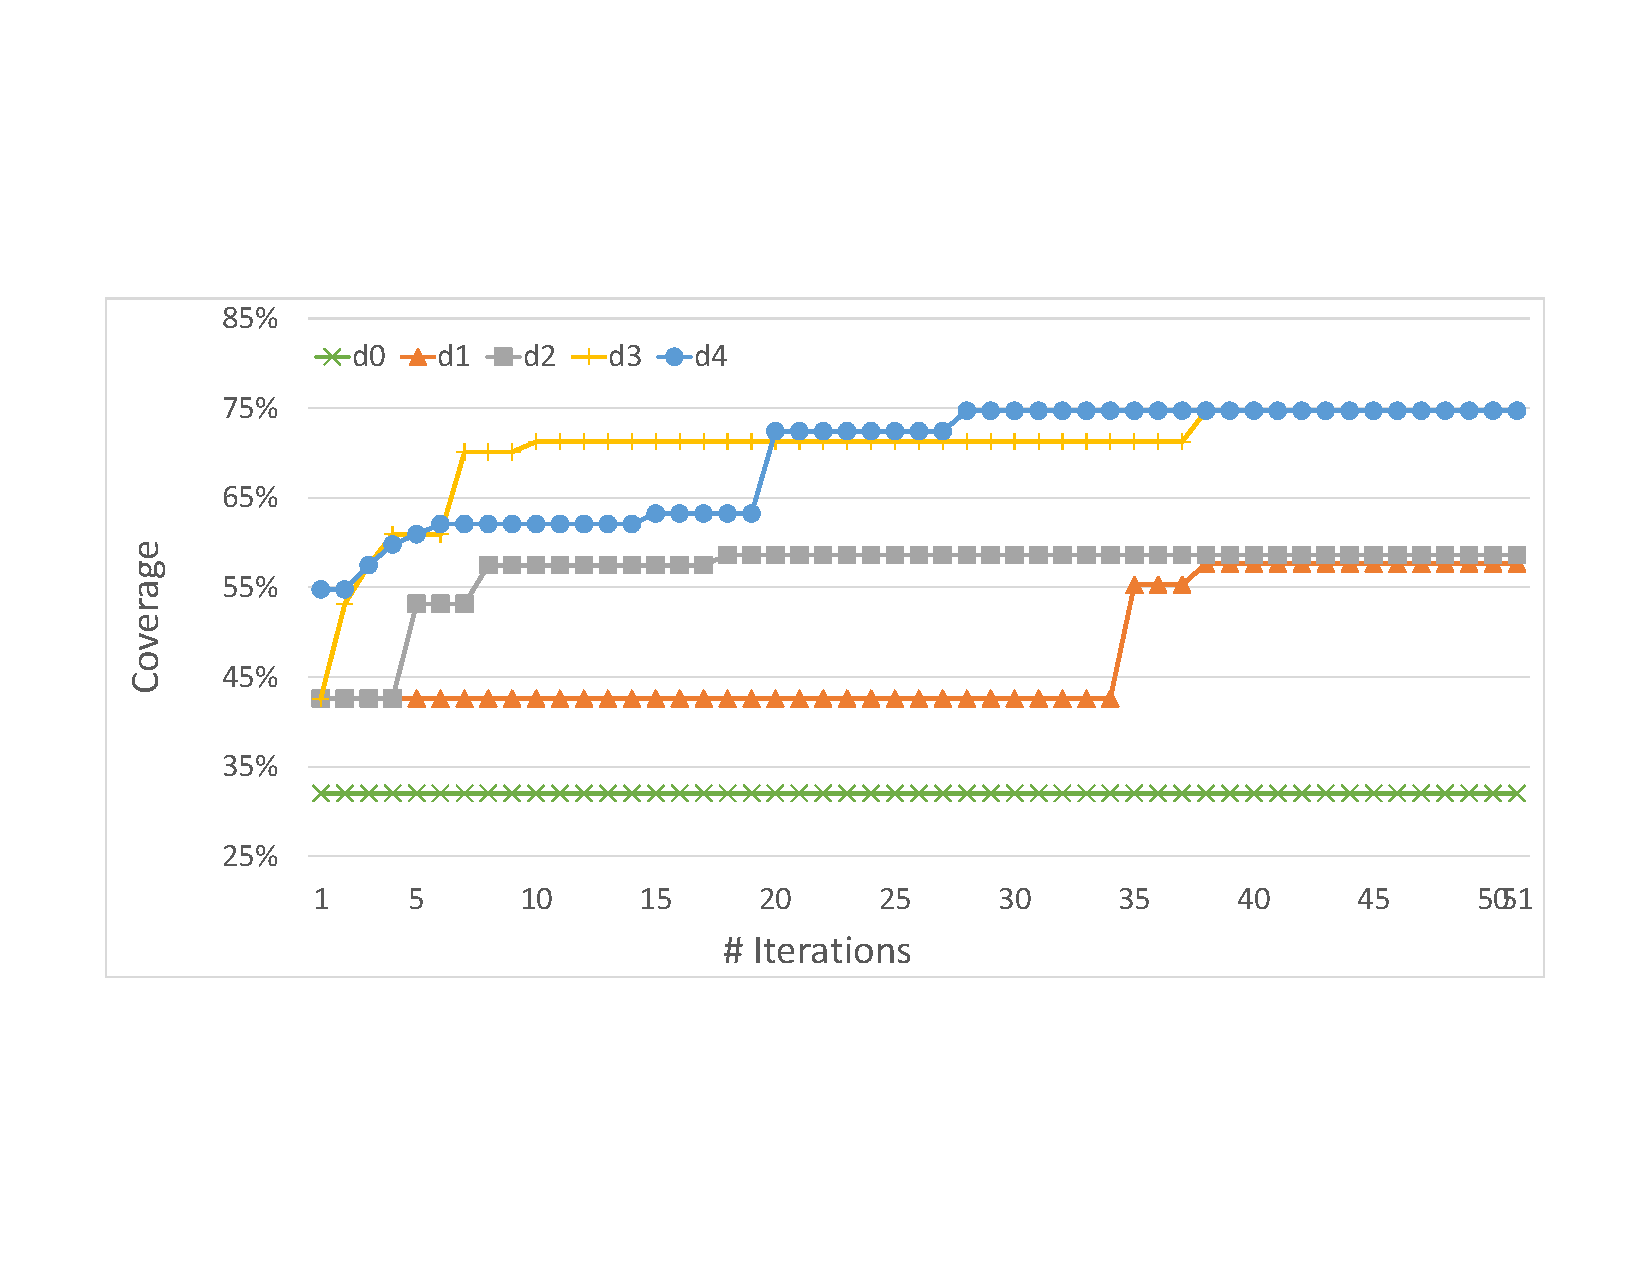
\includegraphics[width=0.8\textwidth]{goat/figs/coverage_etcd7443.pdf}

   \caption{Coverage percentage after each iteration of \goat with various $D$ values for \texttt{etcd7443}. Iterations on the X axis of figures end when the respective bug is first detected.}
   \label{fig:etcd_coverage}
\end{figure}

\begin{figure}[]

       \centering
       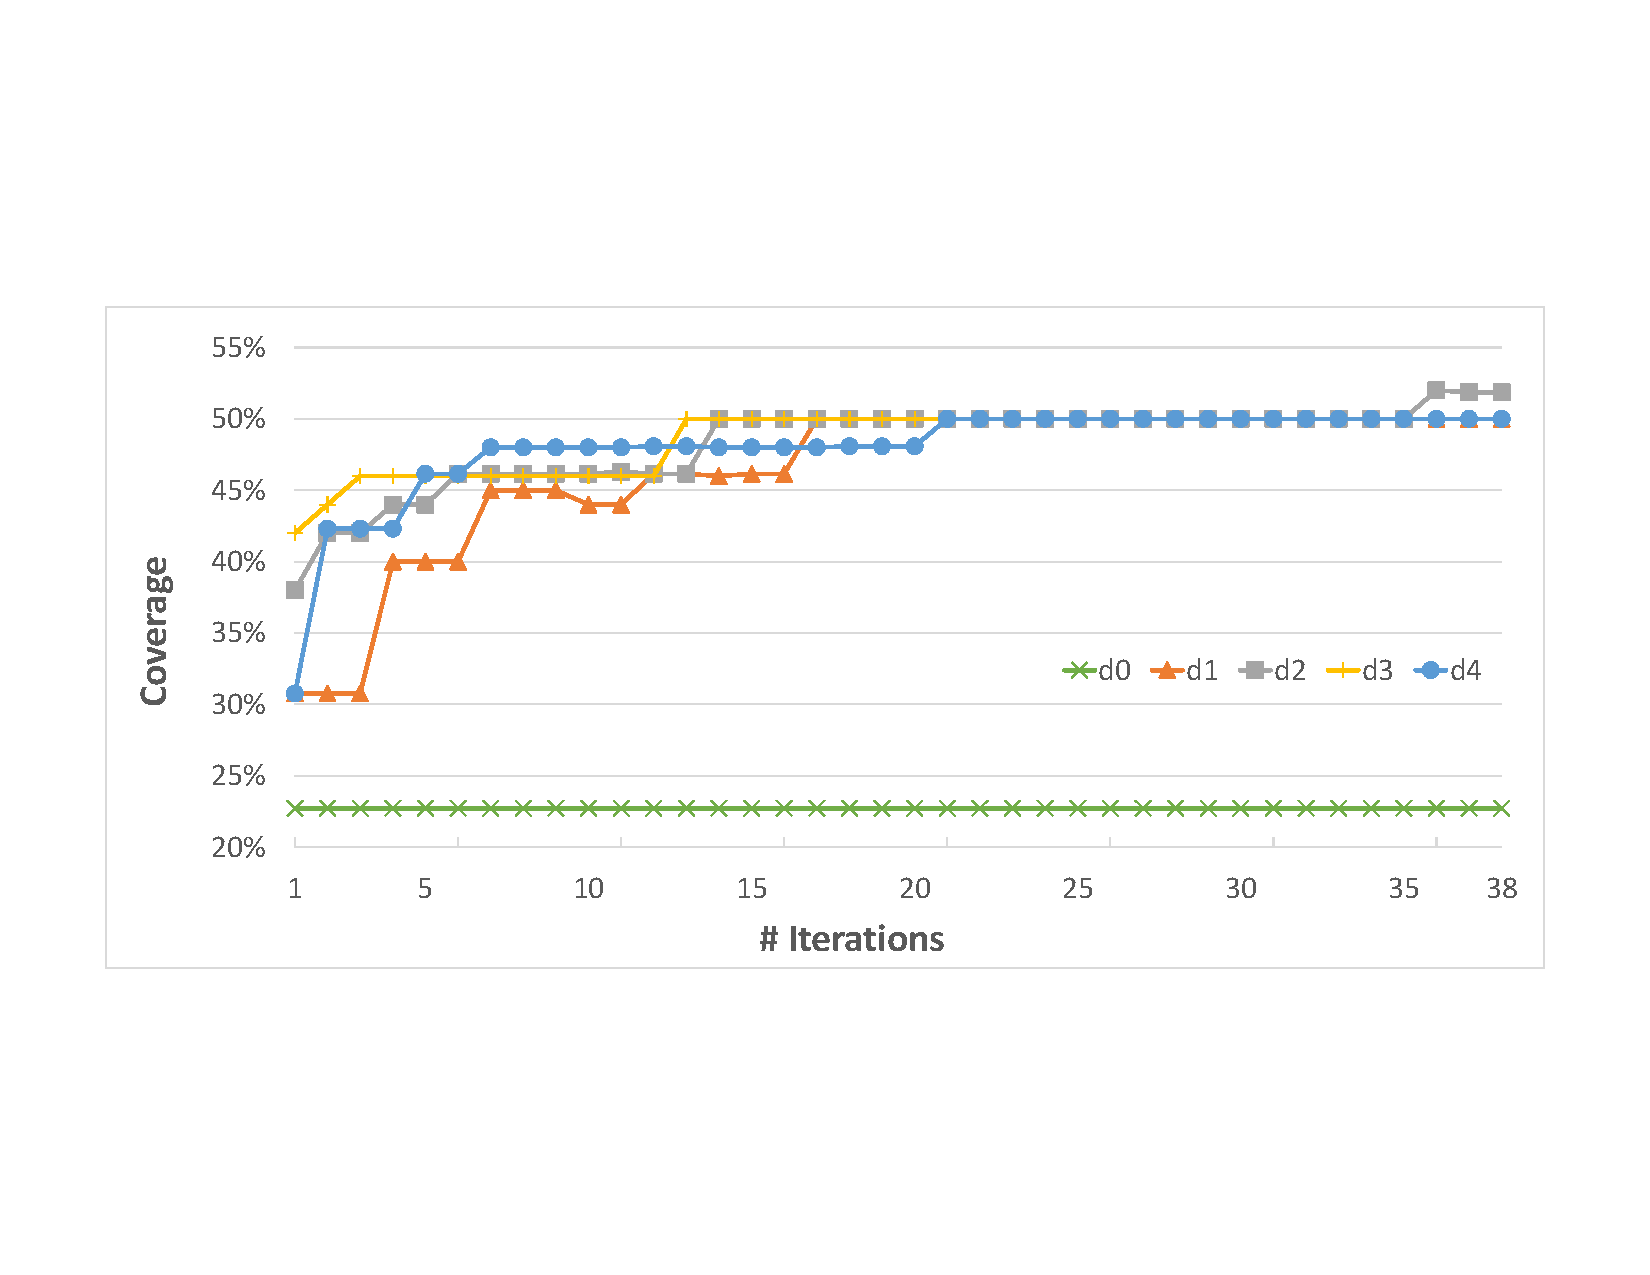
\includegraphics[width=.8\textwidth]{goat/figs/coverage_kubernetes11298.pdf}

       \caption{Coverage percentage after each iteration of \goat with various $D$ values for \texttt{kuberenetes11298}. Iterations on the X axis of figures end when the respective bug is first detected. For example, \goat($D2$) detects the bug in \texttt{kuberenetes11298} after 38 executions at 52.23\% coverage percentage.}
       \label{fig:kubernetes_coverage}

\end{figure}
